% === Impact / Lifetime
\FloatBarrier
\section{\review{Impact of Decapolar Fields}}

Decapolar fields can influence the beam lifetime in several ways. Chromatic amplitude detuning and
chromaticity will induce a tune shift, relative to either or both the action and the momentum
offset. After such detuning, particles may move closer to certain resonances in tune space, causing
their oscillations to grow, eventually leading to their loss.


% ============================================
%                 Large RDT
% ============================================
\subsection{\review{Large RDT}}

\begin{wraptable}{r}{0.4\textwidth}
    \centering
    \begin{tabular}{rr}
    \toprule
    $\Delta K_5$         & RMS $|f_{1004}|$ \\
    \midrule
    $0$                  &            $618,947$ \\
    $\pm10500$             &         $17,566,377$ \\
    $\mp10500$             &         $17,623,867$ \\
    \bottomrule
    \end{tabular}
    \caption{RMS of $|f_{1004}|$ relative to the powering scheme of decapolar correctors.}
    \label{table:decapoles:impact:rdt_amplitude}
\end{wraptable}

As seen previously in \cref{fig:decapoles:rdts:tune_diagram}, the resonance $1Q_x - 4Q_y$ passes
through the beam in tune space, deteriorating the lifetime of the nearby particles.
In order to measure the impact of this resonance on the beam, a knob was created, alternating the 
current of all decapole correctors in the machine arc by arc. Such a powering scheme has no impact
on chromaticity as the sum of the strengths $K_5$ is zero. Rather, the RDT $f_{1004}$ is impacted.
Is it to be noted that this is not a correction, but purely a way to artificially increase the RDT
in order to quantify the effect of the resonance.

Starting with nominals corrections for $Q'''$ corrections, a delta of $\pm 10500 K_5$ is applied on
each decapolar correctors. \Cref{fig:decapoles:impact:alternating_knob} shows the response of the
real part of the RDT for this scheme and its inverse. The amplitude of the RDT is on a similar level
as the shift is significantly larger than the original level of the RDT.
\Cref{table:decapoles:impact:rdt_amplitude} indicates the amplitude of the RDT created with each
knob value.

\begin{figure}[!htb]
    \centering
    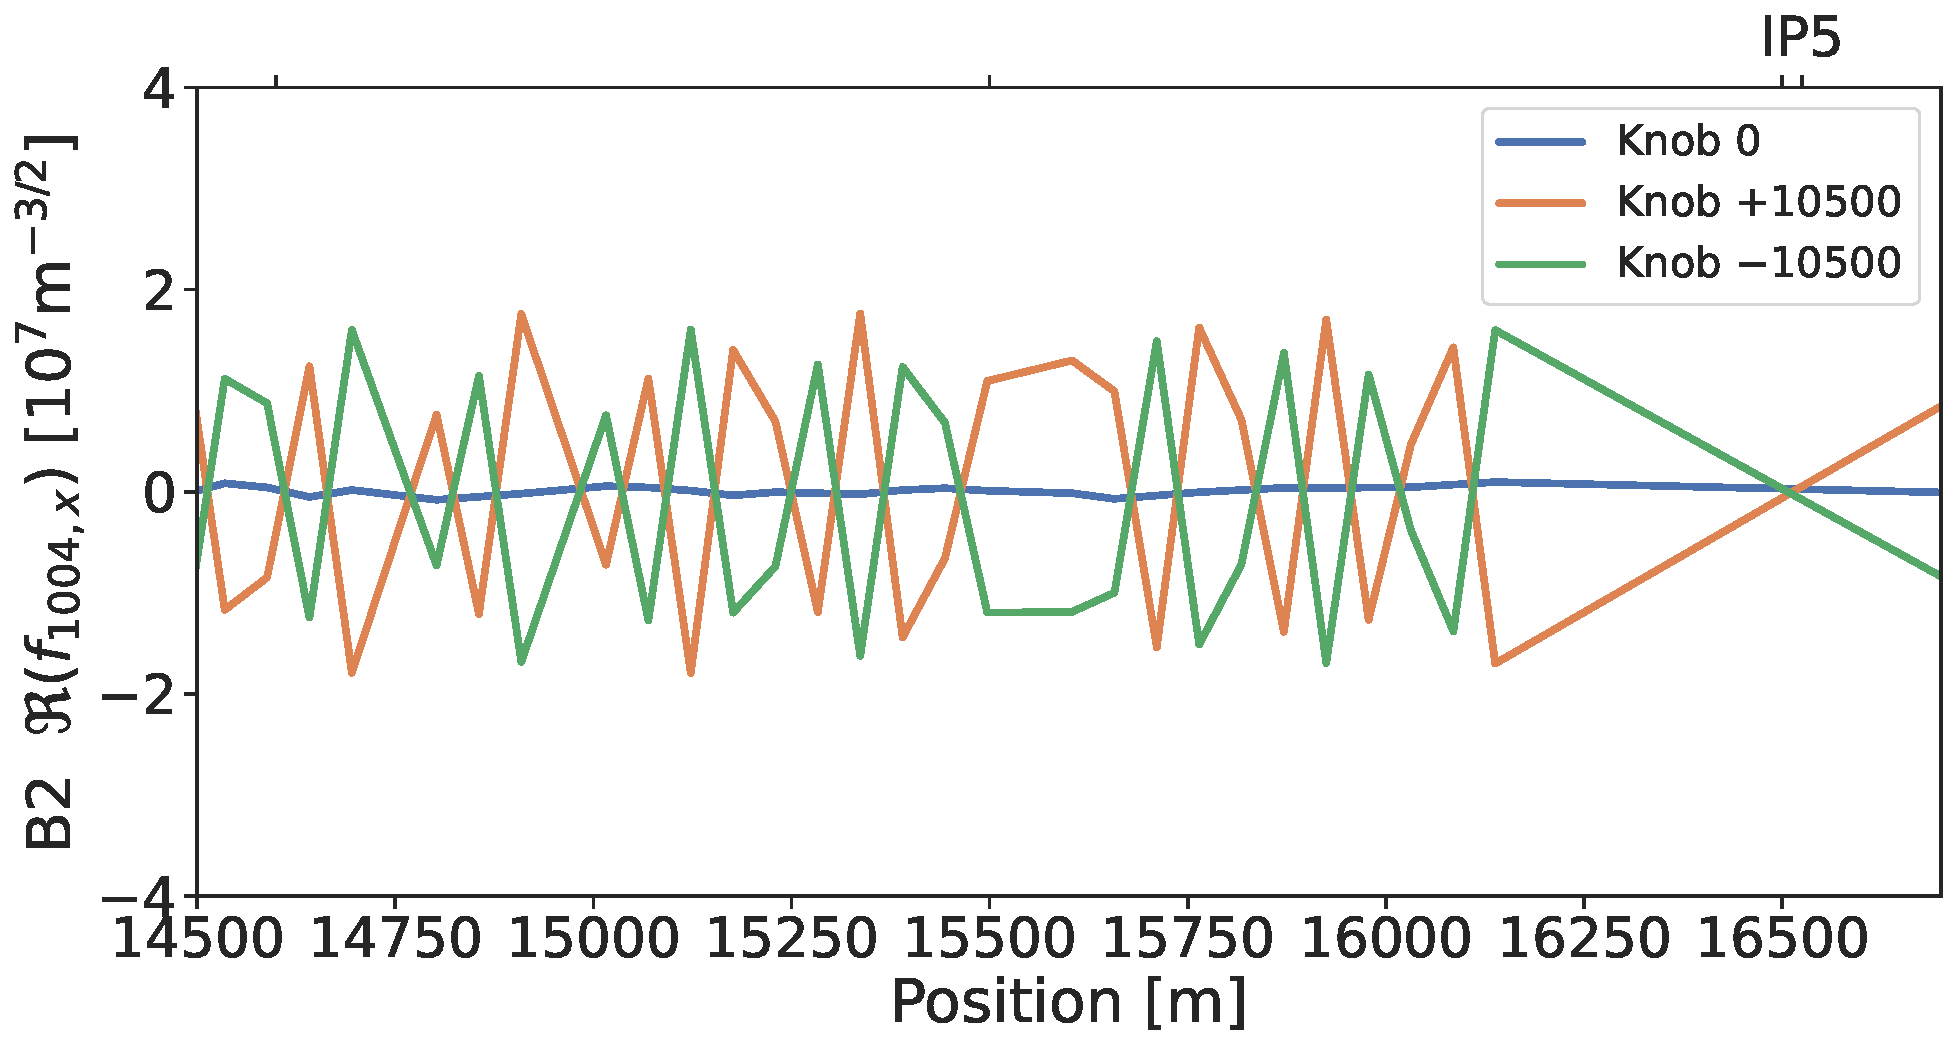
\includegraphics[width=0.8\textwidth]{./images/f1004/f1004x_knob_alt_lifetime_real.pdf}
    \caption{Measured real part of the RDT $f_{1004}$ depending on the powering scheme of the decapolar
    correctors.}
    \label{fig:decapoles:impact:alternating_knob}
\end{figure}

In order to measure the lifetime, a long period must be allocated as the signal returned from
monitors can be jittery. \Cref{fig:decapoles:impact:b5_lifetime} shows this lifetime depending on
the decapolar strength scheme applied. The current of only one circuit is shown for readability.
A current of $\approx 230$ corresponds to a knob value of $+10500$ while a current of $-45$
corresponds to $0$.

\begin{figure}[!htb]
    \centering
    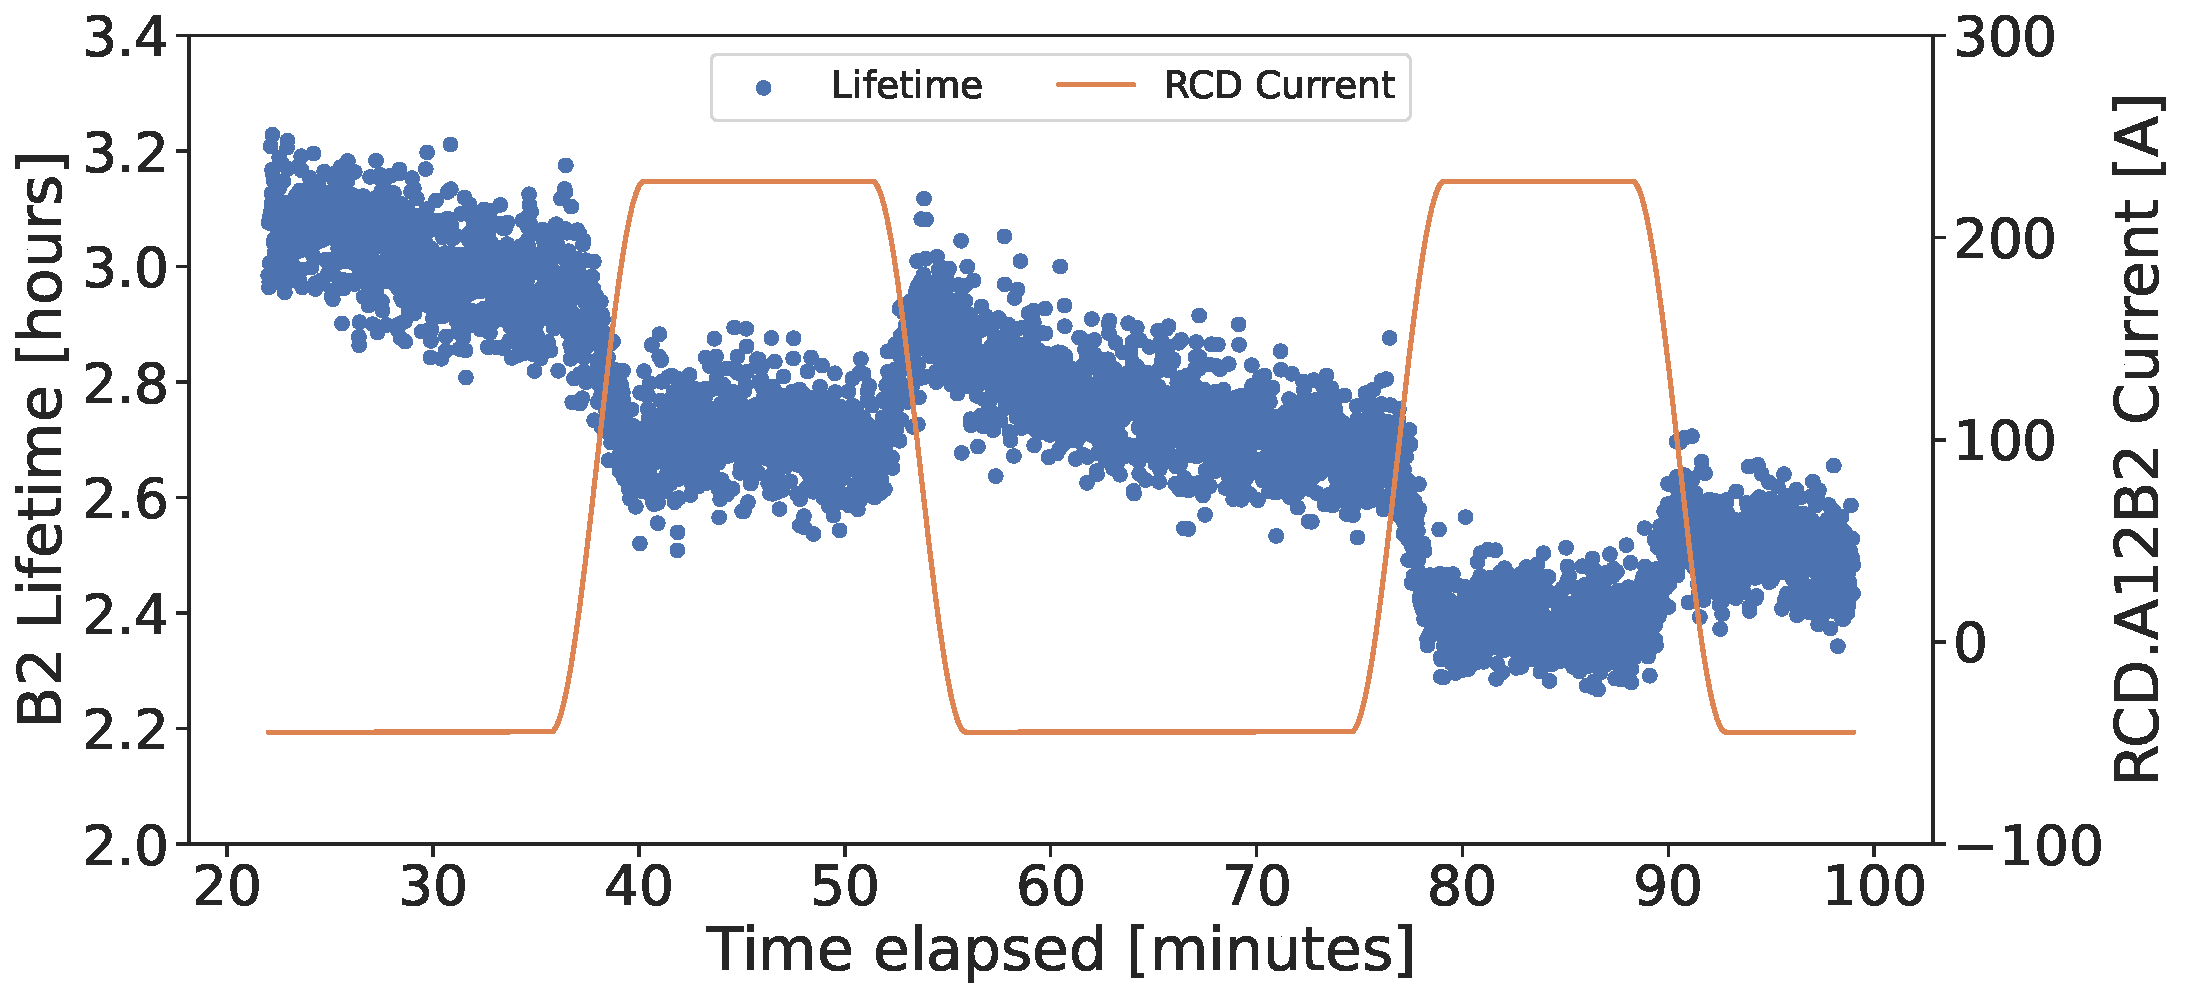
\includegraphics[width=0.8\textwidth]{./images/b5_lifetime.pdf}
    \caption{Measured lifetime of Beam 2 upon application of two different powering schemes for
    decapolar correctors. One trim keeps the RDT at a low amplitude while the other greatly
    amplifies it.}
    \label{fig:decapoles:impact:b5_lifetime}
\end{figure}

It is clear from this measurement that a large RDT decreases the lifetime of the beam.
The first pair of trim sees the average lifetime decreasing of $0.31 \pm 0.03$ hours, while the
second one sees a decrease of $0.36 \pm 0.03$ hours. This observed decrease of 20 minutes accounts
for $10\%$ of the beam lifetime at injection energy.



% ============================================
%                Corrections
% ============================================
\subsection{\review{Corrections}}

In order to understand what can be gained from correcting decapolar fields, a lifetime measurement
was taken with the corrections described in 
\cref{section:decapoles:decapolar_contribution_correction}. This scheme corrects the three decapolar 
observables, being the RDT $f_{1004}$ linked to the resonance $1Q_x - 4Q_y$, the third order
chromaticity $Q'''$ and the chromatic amplitude detuning terms.
\Cref{fig:decapoles:impact:b5_lifetime_rdt_corr} shows the evolution of the lifetime, starting with
corrections applied, removed and then trimmed to their opposite. A net change in lifetime for Beam 1
can be measured after each application. Acquired signal for Beam 2 has been deemed too noisy to be 
relevant, due to the shortness of the measurement.

\begin{figure}[!htb]
    \centering
    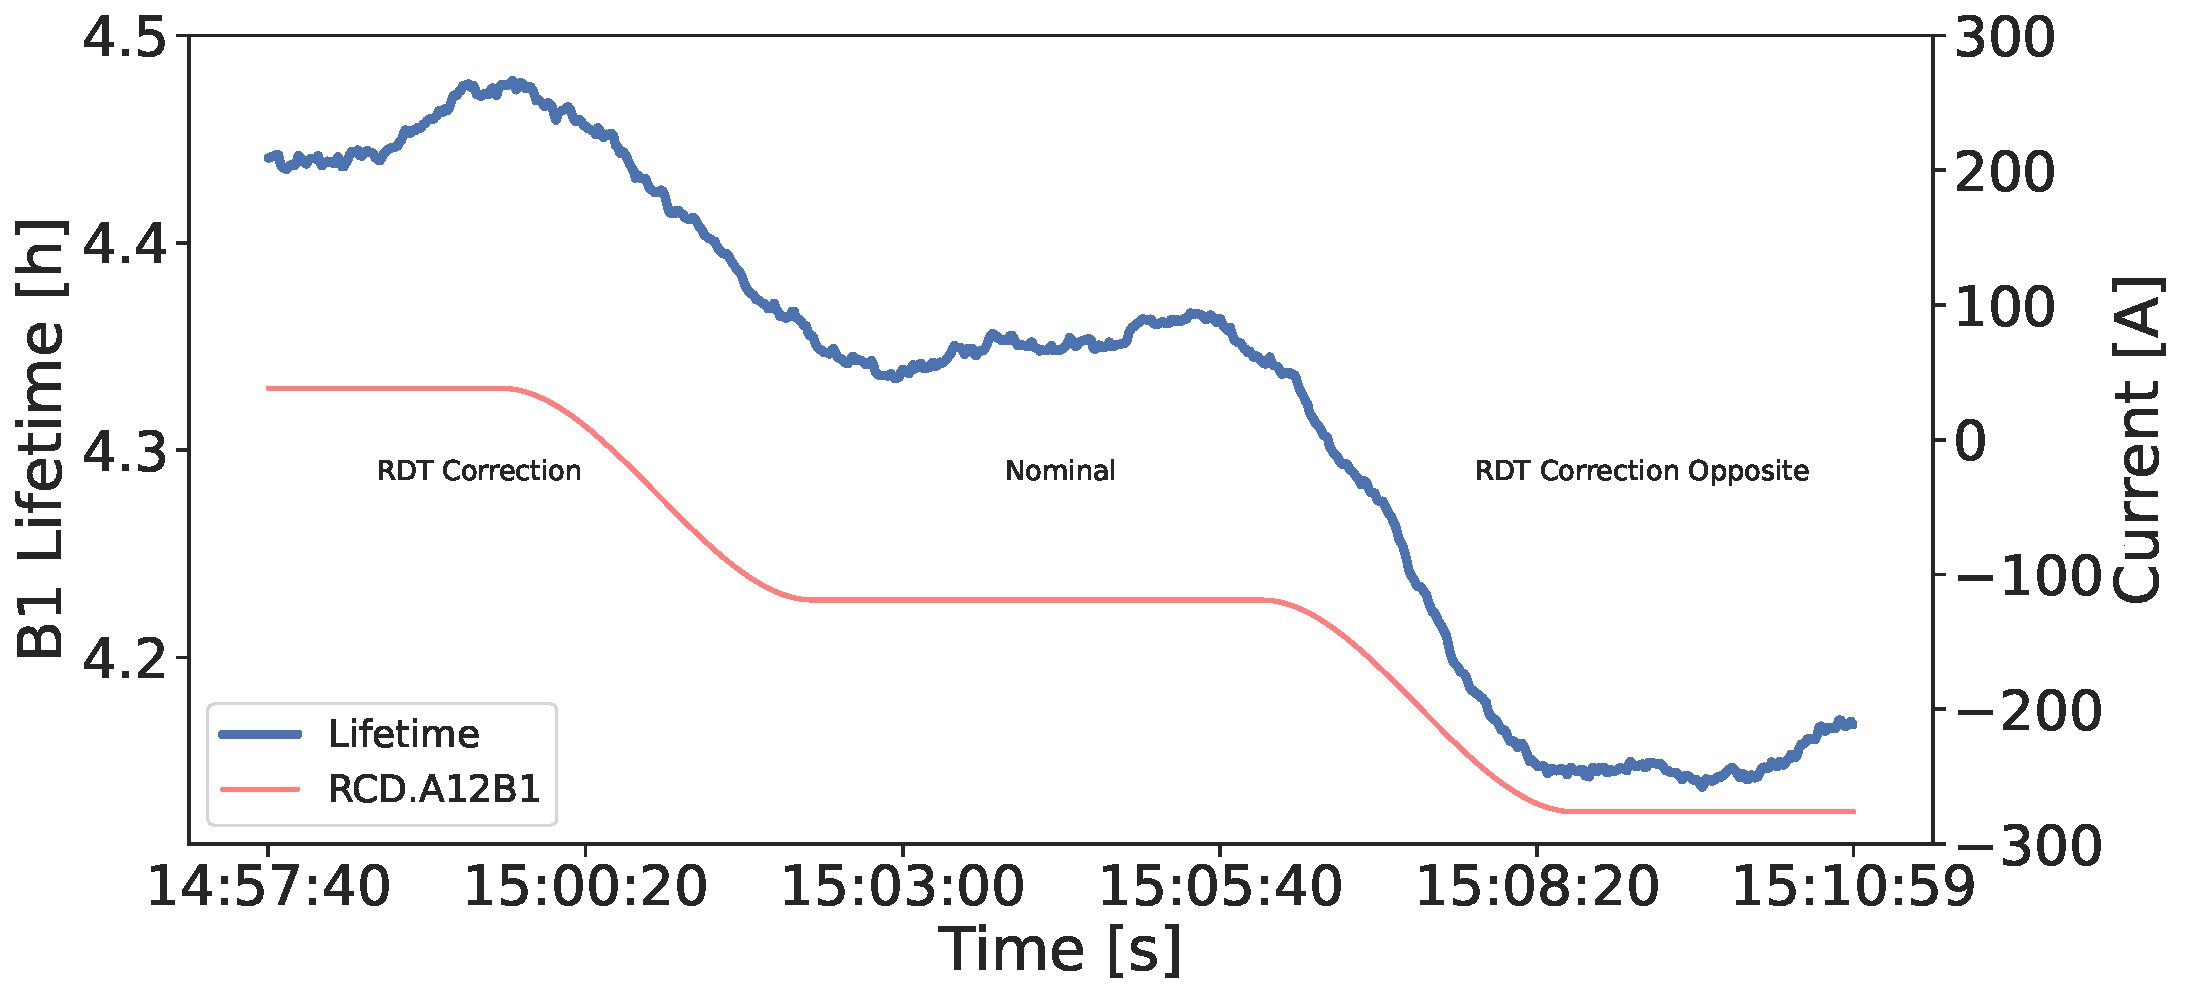
\includegraphics[width=0.8\textwidth]{./images/b5_lifetime_rdt_corr.pdf}
    \caption{Measured lifetime of Beam 1 with the nominal corrections for $Q'''$, combined
    correction of $f_{1004}$ and $Q'''$, and its inverse.}
    \label{fig:decapoles:impact:b5_lifetime_rdt_corr}
\end{figure}

It is apparent here that the corrections have a beneficial effect on the beam. The lifetime
improvement is of $\approx 3 \%$, while the degradation after applying the opposite is of $\approx
5\%$. Further developments in the correction scheme and lengthier measurements could easily improve
this lifetime gain.


Furthermore, a significant improvement in the forced dynamic aperture during AC-Dipole excitation
was observed when corrections were applied. The earlier corrections for decapolar fields were
implemented alongside octupolar corrections for $Q''$. \Cref{fig:decapoles:losses_b4b5_corrs}
demonstrates the relative losses encountered when kicking at different amplitudes with the
AC-Dipole. This clearly shows that octupolar and decapolar corrections enhance the forced dynamic
aperture.

\begin{figure}[!htb]
    \centering
    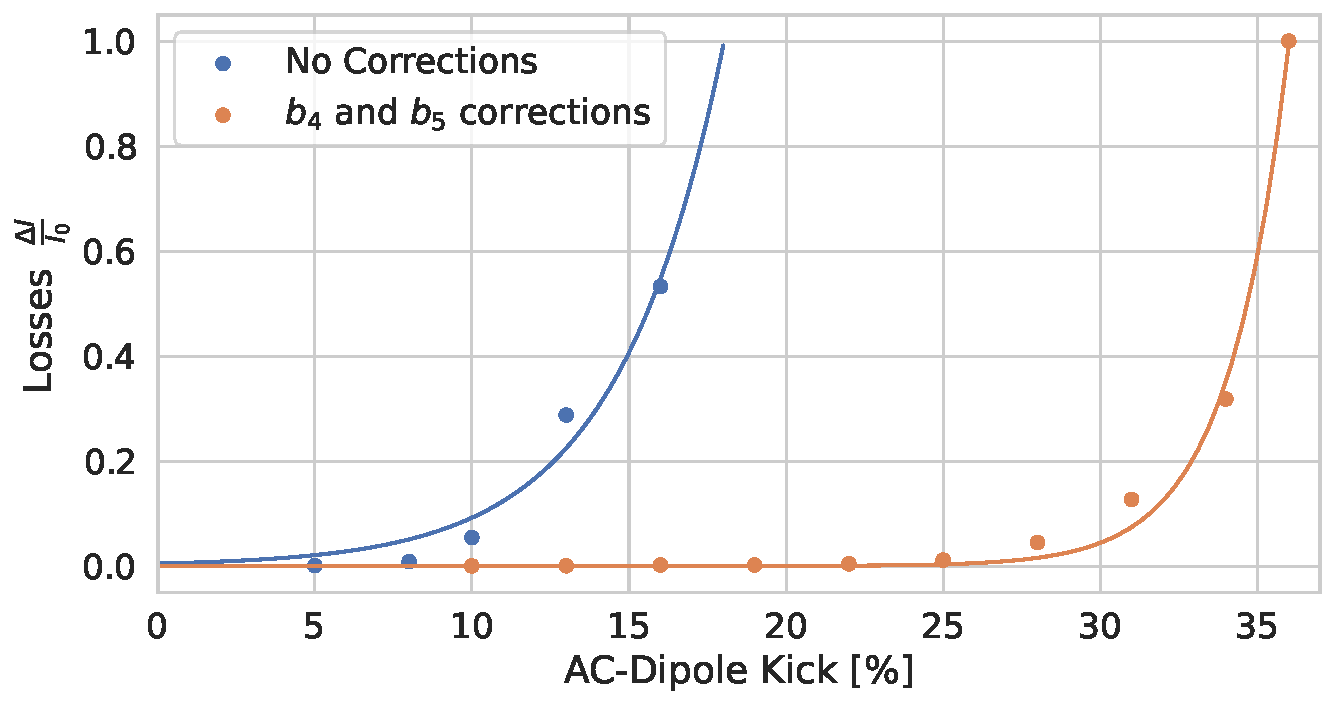
\includegraphics[width=0.8\textwidth]{./images/losses_with_without_b4b5corr.pdf}
    \caption{Relative losses experienced with AC-Dipole kick amplitude with and without corrections
    pertaining to $Q''$, $Q'''$, chromatic amplitude detuning, and RDT $f_{1004}$.}
    \label{fig:decapoles:losses_b4b5_corrs}
\end{figure}

\FloatBarrier